\section{Příklad 3}
% Jako parametr zadejte skupinu (A-H)
\tretiZadani{H}
\noindent\makebox[\linewidth]{\rule{\textwidth}{0.3pt}}\\
Nejdříve si jednotlivé uzly označíme a určíme směry jejich proudů.\\
\begin{center}
    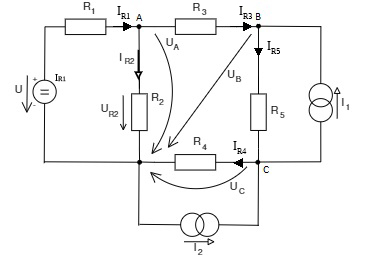
\includegraphics{IEL3.jpg}
\end{center}
Nyní si sestavíme rovnici našich označených uzlů.

$$\boldsymbol{A:} I_{R_1}-I_{R_3}-I_{R_2}=0$$
$$\boldsymbol{B:} I_{1}+I_{R_3}-I_{R_5}=0$$
$$\boldsymbol{C:} -I_{1}+I_{2}+I_{R_5}-I_{R_4}=0$$
\pagebreak
\\
Ještě než začneme počítat si zjistíme vzorce pro jednotlivé proudy pomocí $U_A, U_B, U_C$:\\
$$I_{R_1}=\frac{U-U_A}{R_1}$$
$$I_{R_2}=\frac{U_A}{R_2}$$
$$I_{R_3}=\frac{U_A-U_B}{R_3}$$
$$I_{R_4}=\frac{U_C}{R_4}$$
$$I_{R_5}=\frac{U_B-U_C}{R_5}$$
Teď si rovnici přepíšeme podle vzorců, které jsme si napsali:\\
$$\boldsymbol{A:} \frac{U-U_A}{R_1}-\frac{U_A-U_B}{R_3}-\frac{U_A}{R_2}=0$$
$$\boldsymbol{B:} I_1+\frac{U_A-U_B}{R_3}-\frac{U_B-U_C}{R_5}=0$$
$$\boldsymbol{C:} -I_1+I_2+\frac{U_B-U_C}{R_5}-\frac{U_C}{R_4}=0$$
Do rovnice dosadíme známé hodnoty a upravíme.\\
$$-6821U_A+1833U_B=-294060$$
$$25U_A-83U_B+58U_C=-1377.5$$
$$28U_B-53U_C=315$$
Rovnici přepíšeme do matice.\\
$$
\left (
\begin{array}{ccc}
6821 & -1833 & 0 & 
25&-83&58&
0&28&-53&
\end{array}
\right ) 
*
\left (
\begin{array}{c}
U_A & U_B & U_C
\end{array}
\right )
=
\left (
\begin{array}{c}
294060 & -1377.5 & 315
\end{array}
\right )
$$
\\
Teď si vypočítáme determinanty matic $D_0$ a $D_A$.
$$
D_0 = 
\begin{vmatrix}
6821 & -1833 & 0 \\
25 &-83&58\\
0 & 28 &-53\\
\end{vmatrix}
=16499550
$$
\\
$$
D_A = 
\begin{vmatrix}
294060 & -1833 & 0 \\
-1377.5 &-83&58\\
315 & 28 &-53\\
\end{vmatrix}
= \frac{1832700675}{2}
$$
\\
Podle Cramerova pravidla vypočítáme $U_A$($U_{R_2}$) \\
$$U_A=U_{R_2}=\frac{D_A}{D_0}=\frac{\frac{1832700675}{2}}{16499550}=55.5379V$$\\
Dopočítáme $I_{R_2}$\\
$$I_{R_2}=\frac{U_{R_2}}{R_2}=\frac{55.5379}{39}=1.4240A$$